\documentclass{beamer}

\usepackage[utf8x]{inputenc}
\usepackage{default}

\begin{document}

\begin{frame}
 Architectures :\\
\begin{itemize}
 \item avec un site
\end{itemize}
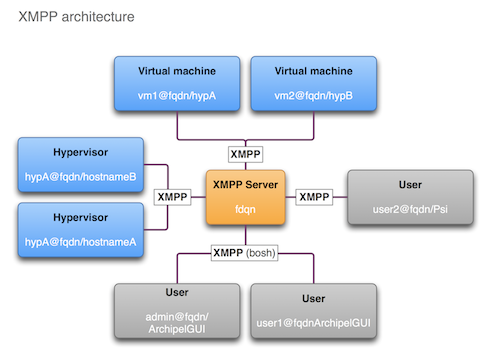
\includegraphics{images_presentation/archipel.png}
\end{frame}

\begin{frame}
\begin{itemize}
 \item avec plusieurs sites
\end{itemize}
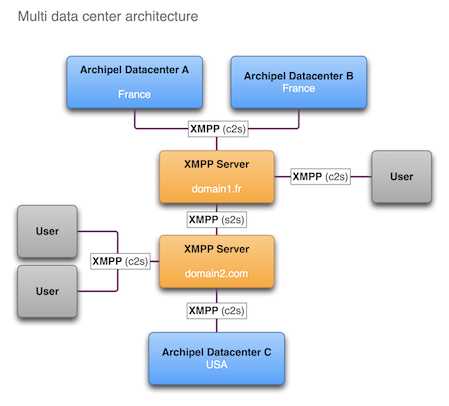
\includegraphics{images_presentation/archipel1.png}
\end{frame}

\begin{frame}
Architecture inetrne:\\
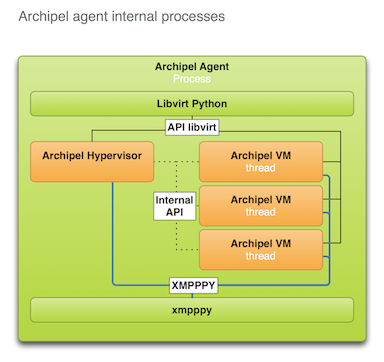
\includegraphics{images_presentation/intern.png}
\end{frame}

\begin{frame}
Fonctionalités : \\
\begin{itemize}
\item Un système de module qui permet d'apporter de nouvelles fonctions
\item La plus part des opérations de base sont disponibles : définition d'une nouvelle VM, manipulations du réseau et du stockage,
accès à la console VNC, gestions des snapshots, etc... 
Les opérations de migration sont également prises en charge
\item Reporting sur l'état de hyperviseur,VMCast, planifications de taches, gestions des droits des
utilisateurs, création d'une machine avec load balacing sur les serveurs
\item Haute disponibilité
\end{itemize}

\end{frame}


\end{document}
